\newpage
\section{System Overview}

\begin{wrapfigure}{r}{0.5\textwidth}%this figure will be at the right
    \centering
    \vspace{-2mm}
    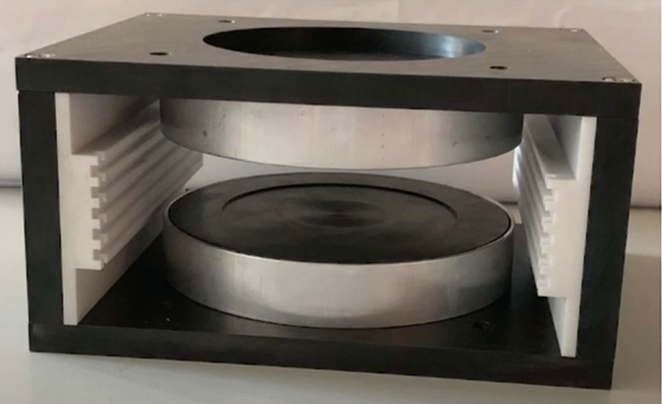
\includegraphics[width=0.48\textwidth]{magnet-interior}
    \caption{\label{fig:magnet} Interior view of the magnet box. Two magnetic disks are held apart with an iron yoke.}
    \vspace{-10mm}
\end{wrapfigure}

There are several components associated with the OCRA tabletop MRI scanner. The primary components are described as follows: 
\vspace{5mm} 

\noindent\textbf{Magnet:} The B0 field is created by a small 0.26T permanent magnet (Figure \ref{fig:magnet}). Two rare-earth magnetic disks are held apart with an iron yoke. The yoke also provides a flux-return path for the magnetic field, containing the magnetic field to the gap between the two poles (and inside the iron). 
\vspace{5mm} 

\noindent\textbf{Phantoms:} A small hole in the top of the magnet serves to accommodate imaging samples. The term \emph{phantom} is used to describe artificial imaging targets.  Next to the scanner you will find several glass tubes to serve as phantoms for this lab.
\vspace{5mm} 

\noindent\textbf{RF coil:}
A radio-frequency (RF) coil encircles the sample bore, serving to transmit the excitation pulse and detect the MR signal through the Faraday detection principle. \textbf{The coil is sensitive to a 20 mm FOV along the bore, centered 15 mm above the bottom of the bore hole}. The coil is a simple solenoid built into an electrical resonator with parallel capacitance so it can be tuned to a specific Larmor frequency. The coil is enclosed by an RF shield consisting of 4 printed circuit boards (PCBs) soldered edge-to-edge (Figure \ref{fig:rf-coil}). The shield acts as a Faraday cage to protect surrounding electronics from RF radiation.

 \begin{figure}[h]
    \centering
    %\vspace{-8mm}
    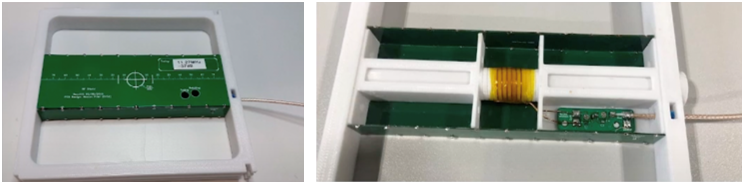
\includegraphics[width=0.9\textwidth]{rf-coil}
    \captionsetup{width=.9\textwidth}
    \caption{\label{fig:rf-coil} (Left) 4 PCBs encase the RF coil to protect surrounding electronics. (Right) RF coil solenoid inside the RF shield.}
    \vspace{-5mm}
\end{figure}

\vspace{5mm}

\noindent\textbf{RF Box:} Inside the magnet box, an RF box (Figure \ref{fig:rf-box-and-grad-filter}, left panel) contains several RF-related components including an RF amplifier, transmit-receive switch, and first \& second stage pre-amplifiers for the received MR signal.  The transmit-receive switch is used to connect the RF coil to the RF amplifier (transmit mode) or low noise pre-amplifier (receive mode).

 \begin{figure}[h]
    \centering
    %\vspace{-8mm}
    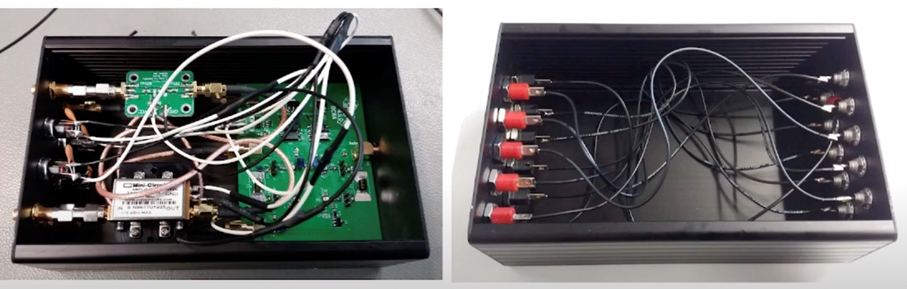
\includegraphics[width=0.9\textwidth]{rf-box-and-grad-filter}
    \caption{\label{fig:rf-box-and-grad-filter} RF box (left) and gradient filter box (right). Both reside in the magnet box.}
    \vspace{-2mm}
\end{figure}

\vspace{5mm}

\noindent\textbf{Gradient System:} The gradient system includes PCB coils, an amplifier, and filter circuitry. The gradient coils (Figure \ref{fig:grad-coils}) generate a spatially varying magnetic field proportional to the current supplied by the amplifier.

\begin{wrapfigure}{r}{0.5\textwidth}%this figure will be at the right
    \centering
    %\vspace{-2mm}
    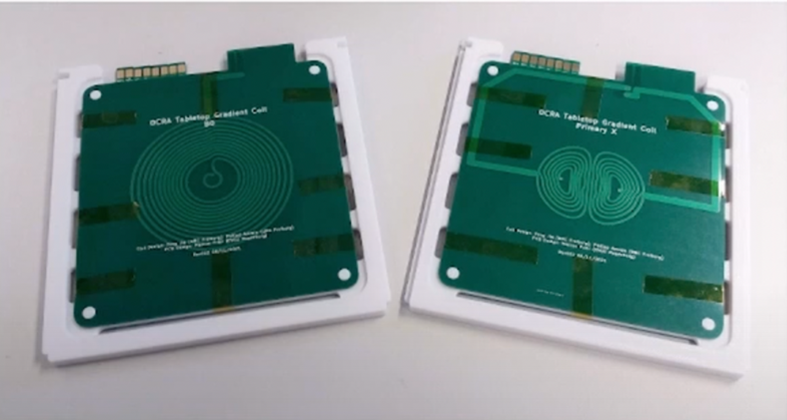
\includegraphics[width=0.48\textwidth]{grad-coils}
    \caption{\label{fig:grad-coils} PCB gradient coils.}
    %\vspace{-5mm}
\end{wrapfigure}

\vspace{5mm}

The gradient amplifier (Figure \ref{fig:grad-amp}) can be viewed as a voltage-to-current transducer: it takes a voltage waveform from the console and creates a current proportional to that voltage in the gradient coil. It is like a common audio power amplifier except that it must also be able to output DC currents.

The gradient amplifier support four channels (X, Y, Z, Z2). The additional channel Z2 is used not for imaging but rather for maintaining homogeneity of the magnetic field.

The amplifier box includes current protection to protect the coils and temperature protection to protect the end stage of each channel. There is also a large power supply and printed circuit boards for the amplifiers.

Filter circuitry (Figure \ref{fig:rf-box-and-grad-filter}, right panel) resides in its own box inside the magnet box, with connections to the gradient channels and feed-through capacitors to shield noise from the gradient amplifier.

\begin{figure}[h]
    \centering
    %\vspace{-8mm}
    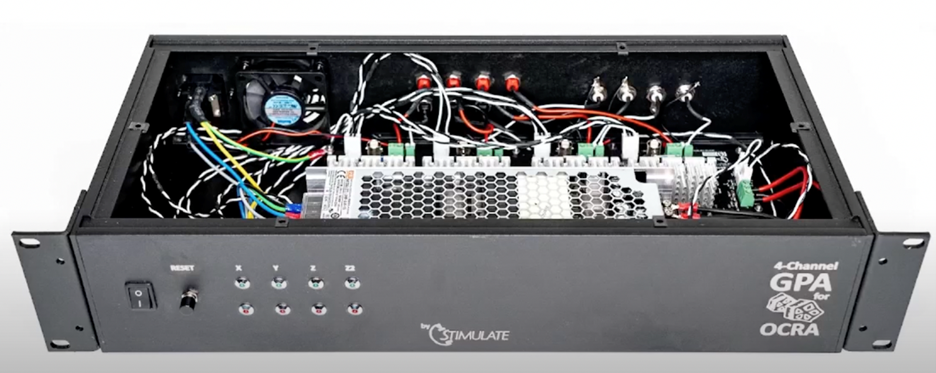
\includegraphics[width=0.9\textwidth]{grad-amp}
    \captionsetup{width=.9\textwidth}
    \caption{\label{fig:grad-amp} Gradient amplifier with X, Y, Z and Z2 channels.}
    \vspace{-2mm}
\end{figure}

\vspace{5mm}

\noindent\textbf{Console:} The console box (Figure \ref{fig:console}) contains two primary components: a Red Pitaya micro-controller and an Ocra1 board (Figure \ref{fig:console-boards}). The Red Pitaya interfaces with a basic MRI console and coordinates signal acquisition by generating RF pulses and control signals for the transmit-receive switch. The MR signal picked up by the RF coil is sampled at an RF input channel through the integrated analog-to-digital converter (RX) on the Red Pitaya. The Red Pitaya is connected to the Ocra1 board which has four 18-bit digital-to-analog converters for gradient waveform generation and an RF attenuator to scale the Red Pitaya output for the RF amplifier input. The console also contains the power supply and a circuit responsible for distributing power among the different parts.

Figure \ref{fig:comms-overview} illustrates the communication pathways between the Red Pitaya, Ocra1, and Raspberry Pi (to be introduced below).

\begin{figure}[h]
    \centering
    %\vspace{-8mm}
    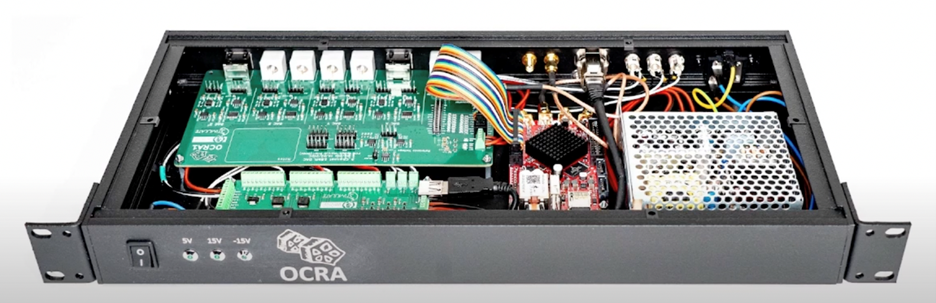
\includegraphics[width=0.9\textwidth]{console-interior}
    \caption{\label{fig:console} Interior view of the console box housing the Red Pitaya micro-controller and the Ocra1 board.}
    \vspace{-5mm}
\end{figure}

\begin{figure}[h]
    \centering
    %\vspace{-8mm}
    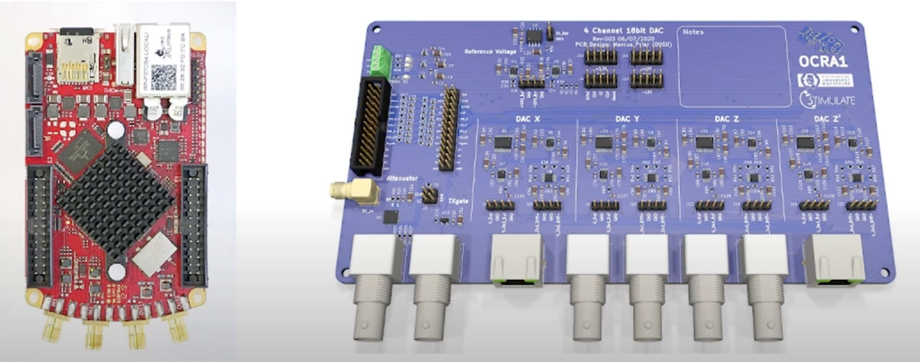
\includegraphics[width=0.7\textwidth]{red-pitaya-and-ocra1}
    \caption{\label{fig:console-boards} Red Pitaya microcontroller (left) and Ocra1 board (right) outside of the RF box.}
    \vspace{-5mm}
\end{figure}

\vspace{5mm} 

\noindent\textbf{Graphical User Interface (GUI):} A Raspberry Pi single-board computer (not pictured - you can find it sitting behind the OCRA stack) allows the user to interface with the tabletop scanner. It hosts a Python program \emph{Relax 2.0} that provides a GUI to interface with the Red Pitaya micro-controller. Basically this program translates Python sequence instructions into RF transmit pulses and gradient waveforms for the lower level hardware to implement.

\begin{figure}[h]
    \centering
    %\vspace{-8mm}
    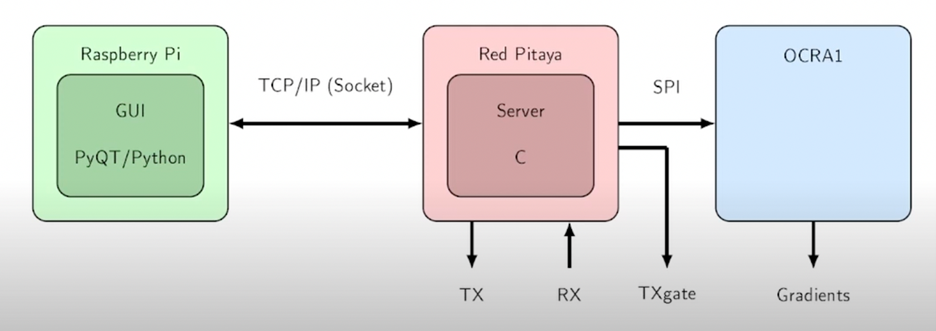
\includegraphics[width=0.9\textwidth]{comms-overview}
    \captionsetup{width=.9\textwidth}
    \caption{\label{fig:comms-overview} Overview of connections between the Raspberry Pi, Red Pitaya, and Ocra1. The Raspberry Pi provides the GUI for the user to change sequence parameters and interact with the system. The Raspberry Pi communicates to the Red Pitaya via a TCP/IP Socket. The OCRA1 extends the Red Pitaya to a basic MRI console via serial peripheral interface (SPI) bus given by the RP GPIO pins. The Red Pitaya coordinates data acquisition by generating RF pulses (TX) and control signals for the transmit-receive switch (TXgate).}
    \vspace{-5mm}
\end{figure}